\documentclass{beamer}

\usepackage{amsmath, amssymb}
\usepackage{tikz-cd}
\usepackage{xcolor}
\usepackage{graphicx}

\title{MAT102 - College Algebra - Polynomial and Rational Functions}
\subtitle{3.2 Introduction to Polynomial Functions \cite{miller2016college}}
\author{\textbf{Miraj Samarakkody}}
\institute{Tougaloo College}
\date{Updated - \today}

\begin{document}

\begin{frame}
    \titlepage
\end{frame}

\begin{frame}
    \frametitle{Determine the End Behavior of a Polynomial Function}

    \begin{block}{Definition of a Polynomial Function}
        Let \(n\) be a natural number and \(a_n, a_{n-1}, \dots, a_1, a_0\) be real numbers, where \(a_n \ne 0\). Then a function defined by \[f(x)=a_n x^n+a_{n-1}x^{n-1}+\dots + a_1 x +a_0\]
        is called a \textbf{Polynomial function of degree \(n\)}. 
    \end{block}\pause
    \vspace{1cm}
    Examples for non-polynomial functions. 


\end{frame}

\begin{frame}
    \frametitle{Several Special Cases of Polynomial Functions}

    Let \(a \ne 0\). \\



\begin{tabular}{lll}
    \(f(x)=c\) & constant function  & degree 0\\
    \(g(x)=ax +b\) & linear function & degree 1 \\
    \(h(x)= ax^2+bx+c\) & quadratic function & degree 2 \\
    \(j(x)=ax^3+bx^2+cx+d\) & cubic function & degree 3 \\
    \(k(x)=ax^4+bx^3+cx^2+dx+e\)& quartic function & degree 4
\end{tabular}
    

\end{frame}

\begin{frame}
    \frametitle{Smoothness and Continuity}
Smooth and Continuous
    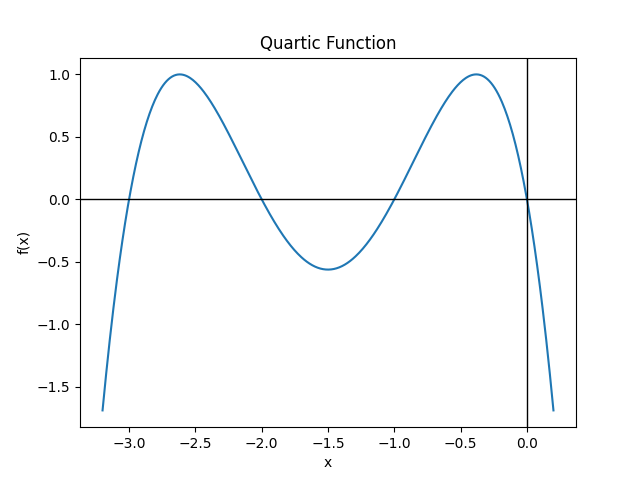
\includegraphics[scale=0.5]{figs/fig_1.png}

\end{frame}

\begin{frame}{Smoothness and Continuity}
    Not Smooth\\
    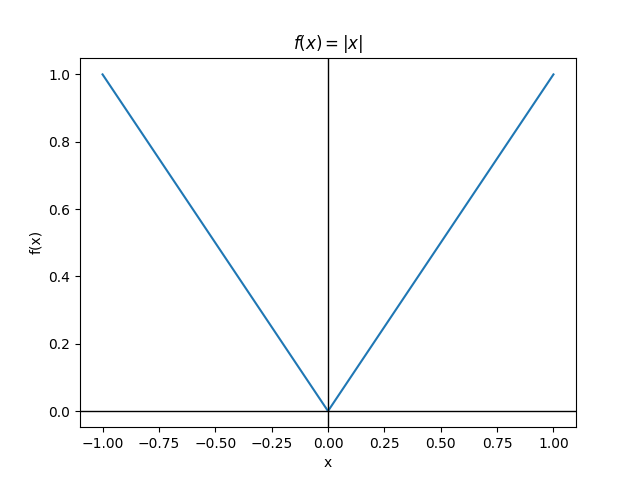
\includegraphics[scale=0.5]{figs/fig_2.png}
\end{frame}

\begin{frame}
    \frametitle{Smoothness and Continuity}

    Not continuous\\
    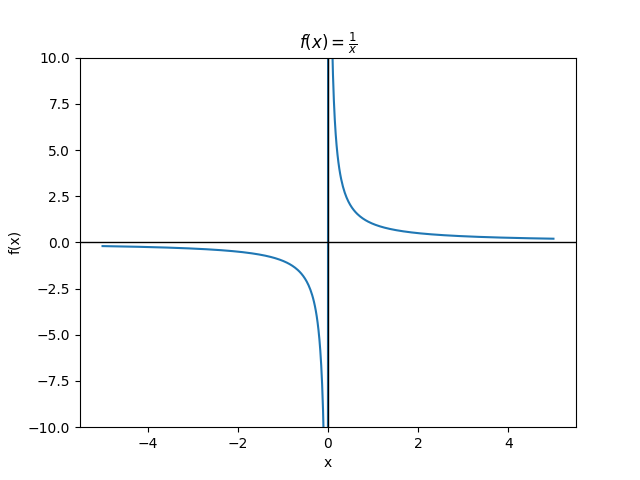
\includegraphics[scale=0.5]{figs/fig_3.png}

\end{frame}

\begin{frame}
    \frametitle{Smoothness and Continuity}

    Not continuous\\

    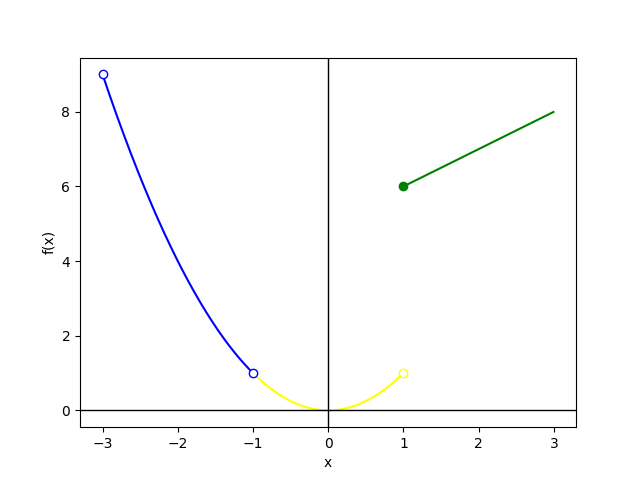
\includegraphics[scale=0.5]{figs/fig_4.png}

\end{frame}



\begin{frame}
    \frametitle{References}
    \bibliographystyle{plain} % or another style like unsrt, alpha, etc.
    \bibliography{reference}  % omit the .bib extension
\end{frame}

\end{document}

